\documentclass[11pt,letterpaper]{article}
\usepackage[utf8]{inputenc}
\usepackage[T1]{fontenc}
\usepackage[spanish]{babel}
\usepackage{lmodern,geometry,setspace,microtype,graphicx,booktabs,longtable,tabularx,array,amsmath,amssymb,float,caption,enumitem,xcolor,hyperref,csquotes,placeins}
\graphicspath{{figuras/}}
% Inserta una gráfica real si existe el archivo; de lo contrario deja un espacio
% visible con el nombre exacto del archivo que debe colocarse en la carpeta figuras/.
\newcommand{\graficaopcional}[5]{%
\begin{figure}[htbp]\centering
\IfFileExists{figuras/#1}{\includegraphics[width=#4,keepaspectratio]{figuras/#1}}{%
\fbox{\begin{minipage}[c][2.0cm][c]{0.88\textwidth}\centering
\textbf{ESPACIO RESERVADO PARA GRÁFICA}\par\vspace{4pt}
Archivo requerido: \texttt{\detokenize{#1}}\par\vspace{4pt}
#5\end{minipage}}}
\caption{#2}\label{#3}
\end{figure}}

\geometry{letterpaper,margin=2.5cm}
\setstretch{1.15}
\setlength{\textfloatsep}{8pt plus 2pt minus 2pt}
\setlength{\intextsep}{8pt plus 2pt minus 2pt}
\setlength{\floatsep}{8pt plus 2pt minus 2pt}
\captionsetup{skip=3pt}
\setlength{\parindent}{1.25cm}
\setlength{\parskip}{0pt}
\renewcommand{\arraystretch}{1.15}
% --- Encabezado: logo (logo.jpeg) solo en la primera página ---
\usepackage{fancyhdr}
\renewcommand{\headrulewidth}{0pt}
\fancypagestyle{plain}{%
  \fancyhf{}%
  \fancyhead[C]{
\includegraphics[height=1.2cm]{logo.jpeg}}%
  \fancyfoot[C]{\thepage}}
\pagestyle{fancy}
\fancyhf{}
\fancyfoot[C]{\thepage}

\hypersetup{colorlinks=true,linkcolor=blue!45!black,citecolor=blue!45!black,urlcolor=blue!55!black}
\title{\textbf{Benchmarking de voz multimodal: evaluación de equidad lingüística}}
\author{Alejandro Agustín Ahedo González \quad Andrés Roberto Osuna González\\[2pt] Sandra Luz Cervantes Espinoza\\[6pt]}
\begin{document}
\maketitle
\begin{center}\small
      \normalsize Proyecto Integrador · Maestría en Inteligencia Artificial Aplicada \\[6pt]
\textbf{Asesoría académica:} Dra. Liliana Ibeth Barbosa Santillán, Dra. Grettel Barceló Alonso y Dr. Luis Eduardo Falcón Morales\\
\end{center}

\begin{abstract}
La expansión de los sistemas de reconocimiento automático del habla (Automatic Speech Recognition, ASR) hace necesario evaluar su desempeño más allá de los idiomas con alta disponibilidad de recursos digitales. Este artículo presenta un estudio comparativo multilingüe cuyo propósito es caracterizar las diferencias de precisión, eficiencia y equidad entre arquitecturas ASR, así como establecer las condiciones necesarias para valorar su transferencia a un entorno operativo. Se empleó el corpus FLEURS y se implementó un flujo reproducible de preprocesamiento y normalización acústica y textual. El análisis exploratorio permitió identificar que una aplicación uniforme de Word Error Rate (WER) produce mediciones engañosas en idiomas cuya escritura no separa palabras mediante espacios; por ello se incorporó Character Error Rate (CER) como métrica comparable a nivel de carácter. En la etapa de comparación de modelos individuales, Whisper-Large-v3 obtuvo el menor WER promedio reportado (4.39\%), seguido por Qwen3-ASR (7.15\%) y SeamlessM4T (7.20\%), mientras que Omnilingual ASR CTC 300M alcanzó 19.28\%. En la etapa de optimización y selección se realizó una evaluación focalizada de Whisper, con particiones independientes de validación y prueba. Los resultados de esa ejecución muestran un CER de 4.91\%, WER de 8.03\% para idiomas con separación por espacios y 1.491 segundos por audio para la configuración greedy. Se proponen decisiones de aceptación, un plan de retroceso metodológico y una arquitectura MLOps para una operación confiable, escalable y auditable.
\end{abstract}
\noindent\textbf{Palabras clave:} ASR, FLEURS, equidad lingüística, WER, CER, Whisper-Large-v3, lenguas de bajos recursos, MLOps.

\section{Contexto de negocio y problema}
\subsection{Organización y motivación}
El estudio se desarrolló en colaboración con CLEAR (Coalition for Language Equity in AI Research), una coalición interdisciplinaria cuyo propósito es promover que las etapas del estudio de inteligencia artificial generativa beneficien también a comunidades hablantes de idiomas subrepresentados. La iniciativa se relaciona con investigación aplicada en tecnologías de voz. El repositorio técnico del equipo se encuentra en \url{https://github.com/Luz026/VoiceBenchmark}.

La motivación central radica en que el desempeño agregado de los sistemas de voz puede ocultar diferencias sustanciales entre idiomas, sistemas de escritura y comunidades de hablantes. Un sistema que presenta resultados favorables en inglés o español no necesariamente mantiene la misma calidad en lenguas con menor presencia en los datos de entrenamiento, alfabetos distintos o convenciones ortográficas diferentes. Esta asimetría puede afectar el acceso a servicios educativos, gubernamentales, de salud e interfaces digitales que dependen de la comunicación oral.

\subsection{Problema y objetivo técnico}
El problema consiste en la ausencia de un procedimiento comparativo homogéneo para evaluar arquitecturas especializadas de voz y modelos multimodales en condiciones multilingües. El proyecto busca medir y caracterizar los errores de transcripción, reconocer patrones de desigualdad y ofrecer criterios reproducibles para seleccionar modelos según idioma, calidad, latencia y costo computacional.

El objetivo general consistió en comparar cuantitativamente modelos de reconocimiento automático del habla utilizandoWER y CER, con énfasis en lenguas de bajos recursos y diferencias asociadas a la arquitectura y al sistema de escritura. La pregunta que orienta la decisión de implementación es: ¿los resultados disponibles son suficientes para implementar el sistema y, si no lo son, qué decisiones deben tomarse antes de avanzar a producción?

\subsection{Evolución del alcance}
El planteamiento inicial contempló una comparación amplia entre modelos especializados (Whisper, SeamlessM4T, Omnilingual y Qwen), además del análisis de acento, dialecto, disponibilidad de recursos lingüísticos y costos de tokenización. El estudio se desarrolló mediante etapas sucesivas y reproducibles. En la etapa de línea base se utilizó Omnilingual ASR CTC 300M como referencia de cobertura amplia, una familia de modelos cuyo trabajo técnico enfatiza la expansión de la cobertura lingüística y la colaboración con comunidades \cite{omnilingual2025}; posteriormente, se compararon cuatro modelos individuales y, finalmente, la optimización experimental se concentró en Whisper-Large-v3, seleccionado a partir de los resultados comparativos previos.

\section{Datos y preparación}
\subsection{Corpus y particionamiento}
El conjunto principal es FLEURS (\textit{Few-shot Learning Evaluation of Universal Representations of Speech}), dataset público, benchmark multilingüe utilizado para tareas de reconocimiento y representación del habla \cite{conneau2023}. La documentación de conjuntos de datos debe acompañar las cifras con procedencia, composición, usos previstos y limitaciones, siguiendo prácticas como las \textit{Datasheets for Datasets} \cite{gebru2021}. La caracterización inicial del corpus describe una cobertura de ciento dos idiomas.

En la etapa de optimización y selección se construyó una evaluación focalizada de ocho idiomas: inglés, español latinoamericano, francés, alemán, italiano, ruso, japonés y chino mandarín. Se descargaron 50 audios por idioma (400 en total) y se separaron 10 por idioma para validación y 10 diferentes para prueba: 80 audios de validación y 80 de prueba.

\begin{table}[H]\centering
\caption{Resumen de conjuntos de datos documentados.}
\begin{tabularx}{\textwidth}{l r X}\toprule
\textbf{Etapa metodológica} & \textbf{Volumen} & \textbf{Uso y observación}\\\midrule
Análisis exploratorio & 5,150 audios; 103 idiomas & 50 audios por idioma, semilla 42.\\
Línea base & 5,087 transcripciones; 102 idiomas & Registros efectivamente evaluados con Omnilingual ASR.\\
Optimización y selección & 400 audios; 8 idiomas & 80 validación, 80 prueba y 240 no utilizados.\\\bottomrule
\end{tabularx}\end{table}

\subsection{Control de calidad y normalización}
El análisis exploratorio confirmó la integridad de los registros estructurales principales y confirmó que los audios se decodificaban correctamente. Identificó, sin embargo, dos riesgos metodológicos: diferencias ortográficas entre referencia y predicción, y uso inadecuado de WER en lenguas sin separación convencional por espacios.

El flujo de procesamiento incluyó el remuestreo a 16 kHz, conversión a canal mono, tipo numérico \texttt{float32}, padding dinámico y batching. La normalización textual utilizó Unicode NFKC, minúsculas y limpieza controlada de puntuación y espacios. Se incluyó mapeo de códigos de idioma cuando las convenciones del modelo no coincidían con los identificadores del corpus, almacenamiento en caché persistente y semilla fija. La preparación reportó que la caché redujo el tiempo de preparación de aproximadamente 106 minutos a menos de un minuto en ejecuciones posteriores. La limpieza debe conservar diacríticos que cambian el significado; no debe aplicarse indiscriminadamente.


\begin{figure}[H]
    \centering
    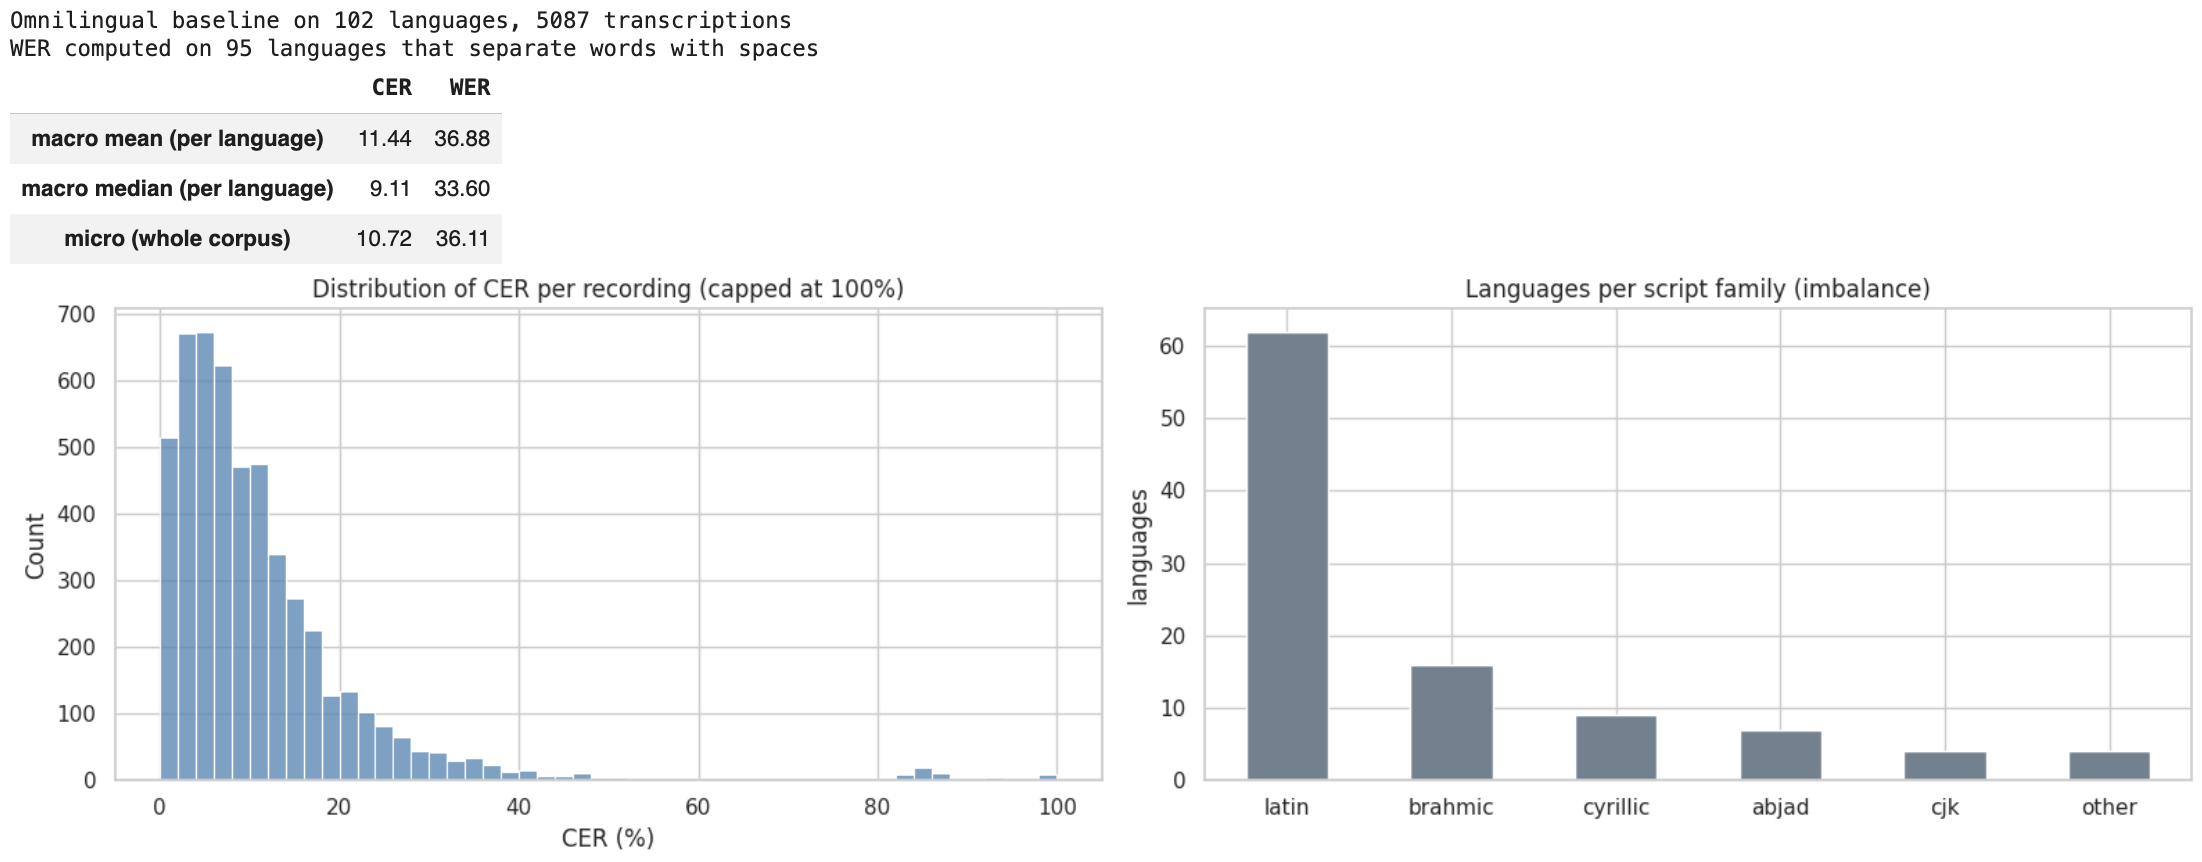
\includegraphics[width=0.85\textwidth]
    {distribucion_idiomas.png}
    \caption{Distribución de muestras por idioma y cobertura del corpus FLEURS.}
    \label{fig:comparacion-modelos-wer}

    \vspace{0.2cm}
    \begin{minipage}{0.9\textwidth}
        \footnotesize
    \end{minipage}
\end{figure}

\subsection{Elección de métricas}
WER se calcula como:
\[WER=\frac{S+D+I}{N},\]
donde $S$, $D$ e $I$ representan sustituciones, eliminaciones e inserciones de palabras y $N$ el número de palabras de referencia. CER utiliza la misma lógica a nivel de carácter:
\[CER=\frac{S_c+D_c+I_c}{N_c}.\]
Ambas métricas pueden superar 100\% cuando existen muchas inserciones. Un WER muy alto no implica necesariamente que el contenido acústico se haya entendido mal si la segmentación de la referencia no corresponde a la del idioma.

La literatura reciente también documenta que WER puede ser inadecuado en idiomas con límites de palabra no explícitos y propone CER como alternativa para evaluación multilingüe \cite{thennal2025}. El caso japonés fue decisivo: durante la etapa de análisis exploratorio, WER calculado con separación por espacios generaba cifras cercanas o superiores al 100\%, aunque la inspección mostraba correspondencia sustancial con el contenido hablado. Al sustituir WER por CER, el error de Whisper-Large-v3 pasó de 74.99\% a 6.21\% en ese análisis inicial. En consecuencia, el protocolo reporta CER para todos los idiomas y WER solo como métrica complementaria donde la segmentación por espacios hace interpretable la comparación.

\section{Metodología y modelos}
\subsection{Diseño experimental}
El trabajo siguió una secuencia inspirada en CRISP-ML(Q), que incorpora aseguramiento de calidad a lo largo de las fases del ciclo de vida de ML \cite{studer2021}: entendimiento del negocio, entendimiento y preparación de datos, modelación, evaluación y consideración de despliegue. Se estableció una línea base, se compararon alternativas y finalmente se optimizó Whisper-Large-v3. La selección de hiperparámetros se realizó sobre validación independiente; el conjunto de prueba se reservó para estimar el rendimiento final.

\subsection{Línea base y diagnóstico predictivo}
En la etapa de línea base, Omnilingual ASR CTC 300M se utilizó como modelo de referencia para la transcripción por su cobertura reportada de 102 idiomas y arquitectura CTC. La ejecución registró CER macro de 11.4\%, mediana de 9.1\% y CER micro de 10.7\%. El WER macro fue 36.9\% en idiomas con separación por espacios. La cobertura de idiomas con CER menor o igual a 10\% fue 52.9\%, con Gini de 0.299 y razón máximo/mínimo de CER de 19.6 veces. Estos resultados evidencian que el promedio global no describe por sí solo la distribución del error.

La misma etapa exploró la predicción del CER mediante características del idioma, audio, texto y hablantes. La varianza del CER se descompuso en 42.5\% entre idiomas y 57.5\% entre grabaciones dentro de cada idioma. Ridge obtuvo $R^2=-0.062$ en prueba y MAE de 0.0762, apenas 1.8\% mejor que el predictor basado en la media (MAE 0.0775). Random Forest de profundidad 8 mostró sobreajuste: $R^2$ de entrenamiento de 0.45 y $R^2$ de prueba de -0.66. La familia de escritura fue el grupo de características más útil; la correlación de Spearman entre ranking predicho y observado de dificultad fue $\rho=0.54$ ($p=3.6\times10^{-9}$). Las características disponibles no bastaron para predecir robustamente el error de cada grabación o generalizar a idiomas no vistos.

\begin{figure}[H]
    \centering
    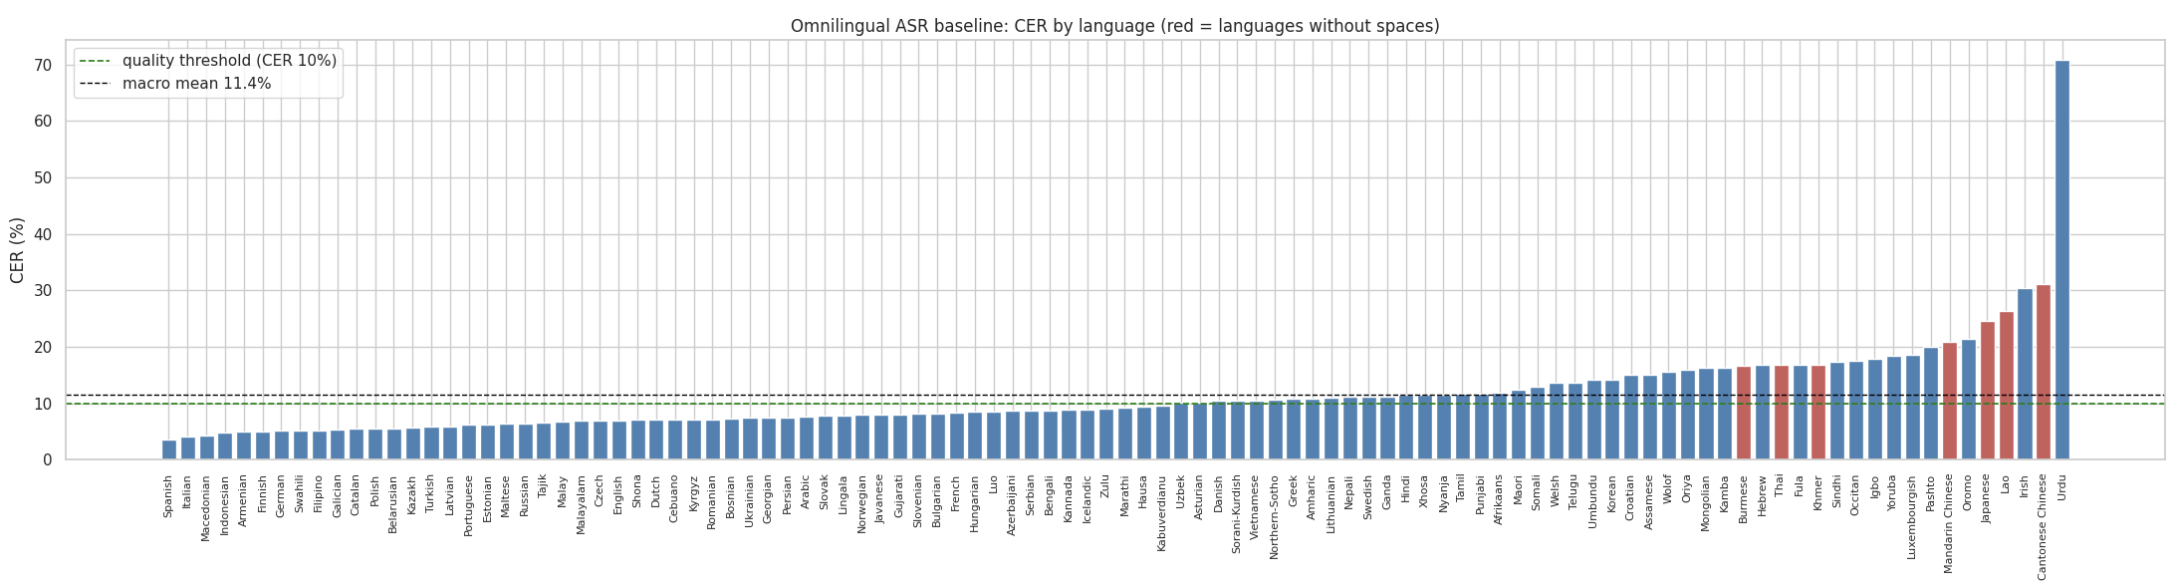
\includegraphics[width=0.85\textwidth]
    {omnilingual_idioma.png}
    \caption{CER de Omnilingual ASR CTC 300M por idioma durante la etapa de línea base.}
    \label{fig:comparacion-modelos}
    \begin{minipage}{0.9\textwidth}
        \footnotesize
    \end{minipage}
\end{figure}

\subsection{Comparación de modelos individuales}
Durante la etapa comparativa se evaluaron Omnilingual ASR CTC 300M, Qwen3-ASR-0.6B, SeamlessM4T y Whisper-Large-v3. El informe técnico de Qwen3-ASR caracteriza la familia y sus capacidades multilingües, aunque sus cifras publicadas no sustituyen los resultados experimentales de este equipo \cite{shi2026}. Las publicaciones de los modelos describen objetivos y capacidades diferentes: reconocimiento multilingüe robusto \cite{radford2023}, traducción y reconocimiento multimodal \cite{seamless2023}, y cobertura extensible de lenguas \cite{omnilingual2025}. Los resultados agregados indican que Whisper-Large-v3 obtuvo el menor WER promedio, 4.39\%; Qwen3-ASR, 7.15\%; SeamlessM4T, 7.20\%; y Omnilingual ASR CTC 300M, 19.28\%. El modelo con mayor cobertura lingüística no necesariamente alcanza la menor tasa de error en el subconjunto evaluado: la selección debe considerar cobertura, precisión y eficiencia.

\begin{table}[H]\centering
\caption{Resultados agregados reportados en la etapa comparativa.}
\begin{tabular}{lr}\toprule\textbf{Modelo} & \textbf{WER promedio}\\\midrule
Whisper-Large-v3 & 4.39\%\\ Qwen3-ASR-0.6B & 7.15\%\\ SeamlessM4T & 7.20\%\\ Omnilingual ASR CTC 300M & 19.28\%\\\bottomrule\end{tabular}\end{table}

La necesidad de desagregar métricas también coincide con estudios de equidad en ASR multilingüe que encuentran disparidades relevantes entre grupos y subgrupos \cite{vanzee2024,swain2024,graham2024}. La evaluación comparativa también identificó variaciones asociadas con el idioma y la familia de escritura. En el análisis de grupos, los idiomas cirílicos y latinos mostraron menores CER agregados que los grupos abjad y CJK. El CER medio reportado para CJK fue 22.7\%, frente a 9.9\% para el grupo latino. La fertilidad de tokenización y el denominado \textit{Tokenizer Tax} se plantearon como dimensiones relevantes para interpretar desigualdades, aunque los documentos no establecen una relación causal generalizable entre fertilidad y error.

\subsection{Optimización y modelo final}
Durante la etapa de optimización y selección se utilizó exclusivamente una arquitectura ASR: \texttt{openai/whisper-large-v3}. No se reentrenaron sus pesos; se compararon estrategias de decodificación sobre el mismo modelo: greedy (\texttt{num\_beams=1}), búsqueda por haces (\texttt{num\_beams=3} y \texttt{num\_beams=5}) y consenso homogéneo por medoide de las tres hipótesis. Se ajustaron parámetros de inferencia, no la arquitectura.

El experimento consideró 400 audios de FLEURS: ocho idiomas con 50 muestras cada uno. Para cada idioma se reservaron 10 audios para validación y otros 10 para prueba no vista; 30 muestras por idioma quedaron sin utilizar. Así, los conjuntos de validación y prueba contienen 80 audios cada uno. La selección de parámetros se realizó con el conjunto de validación y favoreció la búsqueda por haces (Beam Search) con \texttt{num\_beams=5} y \texttt{length\_penalty=1.0}. En el procedimiento final de selección, que compara greedy, Whisper optimizado y consenso homogéneo sobre la prueba, la configuración seleccionada fue Whisper-Large-v3 con decodificación greedy, de acuerdo con el criterio programado de CER y desempate por tiempo. La configuración seleccionada obtuvo CER de 4.91\%, WER de 8.03\% en idiomas con separación por espacios, coincidencia exacta de 33.75\% y tiempo promedio de 1.491 s/audio. En consecuencia, Beam Search con cinco haces obtuvo el mejor resultado durante la validación, mientras que la estrategia greedy fue seleccionada por el procedimiento final aplicado al conjunto de prueba; no deben confundirse ambos resultados. Esta etapa de optimización y selección no presenta una evaluación ejecutada de Qwen3-ASR, SeamlessM4T, Wav2Vec2 ni de ensambles heterogéneos.

\begin{table}[H]\centering
\caption{Resultados reportados por el bloque de selección final de etapa de optimización y selección.}
\begin{tabularx}{\textwidth}{Xr}\toprule\textbf{Indicador} & \textbf{Resultado}\\\midrule
Arquitectura & Whisper-Large-v3\\
Estrategia seleccionada en prueba & Greedy (base)\\
Configuración con mejor resultado en validación & Beam Search, \texttt{num\_beams=5}\\
CER en prueba (greedy) & 4.91\%\\
WER en idiomas con espacios (greedy) & 8.03\%\\
Coincidencia exacta (greedy) & 33.75\%\\
Tiempo promedio (greedy) & 1.491 s/audio\\
Tamaño del conjunto de prueba & 80 audios, 8 idiomas\\\bottomrule\end{tabularx}\end{table}

\begin{figure}[H]
    \centering
    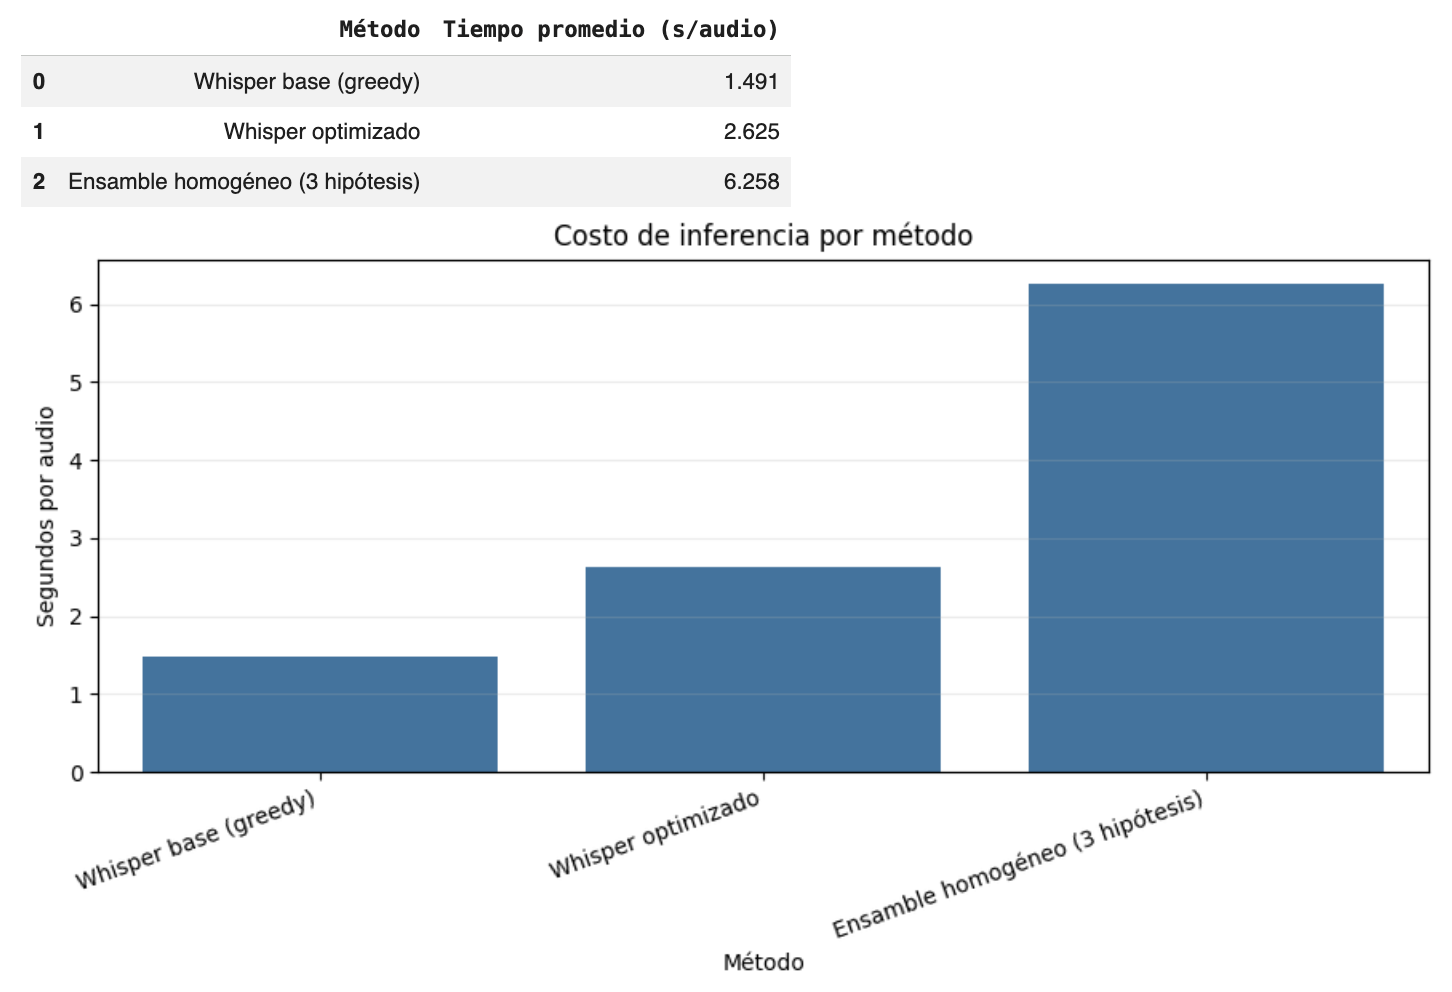
\includegraphics[width=0.85\textwidth]
    {validacion_whisper.png}
    \caption{Comparación en prueba no vista entre greedy, Beam Search optimizado y consenso medoide,
todos basados en Whisper-Large-v3.}
    \label{fig:comparacion-whisper}
    \begin{minipage}{0.9\textwidth}
        \footnotesize
    \end{minipage}
\end{figure}

La coincidencia exacta es más estricta que CER o WER: una transcripción puede contener pocos errores de carácter y aun así no coincidir exactamente con la referencia. El valor de 33.75\% no debe interpretarse como exactitud de clasificación ni como equivalente a $1-CER$.
\section{Resultados y validación}
\subsection{Lectura del desempeño}
Los resultados de la etapa de optimización y selección respaldan la consideración de Whisper-Large-v3 como candidato para un piloto controlado en el subconjunto evaluado; sin embargo, no acreditan todavía su preparación para un despliegue general en producción. En la etapa comparativa, Whisper-Large-v3 obtuvo el menor WER promedio entre los cuatro modelos individuales evaluados (4.39\%); ese dato pertenece a una etapa y protocolo distintos. En la etapa de optimización y selección, el procedimiento final seleccionó la estrategia greedy y obtuvo 4.91\% CER, 8.03\% WER en idiomas segmentables por espacios, 33.75\% de coincidencia exacta y 1.491 segundos por audio.

Desde la perspectiva de aplicación, una sustitución puede alterar nombres propios, cifras o términos especializados; una eliminación puede omitir información; y una inserción puede introducir contenido no expresado. En escenarios de alto impacto, un error pequeño puede modificar el sentido de una instrucción. La aceptación no debe depender únicamente del CER promedio: también debe considerar criticidad semántica, revisión humana y comportamiento por idioma.

\subsection{Umbrales de aceptación propuestos}
Para convertir los resultados experimentales en decisiones operativas, se proponen umbrales iniciales de piloto, sujetos a aprobación de CLEAR y de los responsables del caso de uso.

\begin{table}[H]\centering
\caption{Criterios de decisión propuestos para un piloto controlado.}
\begin{tabularx}{\textwidth}{p{0.22\textwidth}XX}\toprule
\textbf{Dimensión} & \textbf{Criterio propuesto} & \textbf{Acción si no se cumple}\\\midrule
Calidad global & CER macro $\leq 8\%$ en conjunto objetivo; WER solo donde sea válido. & Revisar normalización, segmentación y configuración; si persiste, volver a modelación.\\
Equidad & Ningún idioma prioritario con CER $>15\%$ sin mitigación explícita. & No habilitar uso autónomo; ampliar datos y evaluar alternativas.\\
Latencia & Percentil 95 compatible con el SLA definido por producto. & Optimizar batching, hardware o decodificación.\\
Robustez & Sin fallos sistemáticos de carga, decodificación o idioma. & Suspender la liberación y corregir el flujo de procesamiento.\\
Gobierno & Trazabilidad de versión, datos, parámetros y métricas; mecanismo de fallback. & No promover a producción hasta completar controles.\\\bottomrule\end{tabularx}\end{table}

Los valores de CER constituyen criterios preliminares de aceptación para el piloto, no un resultado experimental. Deben revisarse por idioma y aplicación: un servicio de búsqueda puede tolerar errores que serían inaceptables en dictado médico, trámites o captura de datos financieros.

\subsection{Limitaciones y validez}

\begin{enumerate}
\item FLEURS contiene grabaciones de lectura relativamente limpias. El desempeño con conversación espontánea, ruido, solapamiento de voces y micrófonos heterogéneos requiere validación adicional.
\item Las etapas comparativa y de optimización proceden de subconjuntos y protocolos diferentes; sus métricas no deben mezclarse en un ranking sin reevaluación común.
\item La validación seleccionó Beam Search con cinco haces, pero el procedimiento final de selección de prueba eligió greedy.
\item Dos audios de prueba de más de 30 segundos (uno alemán y uno italiano) generaron excepciones por el manejo de generación larga; el código sustituyó esas salidas por cadenas vacías. Se requiere corregir el tratamiento de audios largos (marcas de tiempo o segmentación) y recalcular métricas. La ejecución en Colab utilizó GPU Tesla T4 con aproximadamente 14.56 GB de VRAM, aunque la configuración experimental recomendaba al menos 16 GB.
\end{enumerate}

\section{Implementación y operación}
\subsection{Decisión de implementación}
Se recomienda proceder con un piloto controlado que utilice Whisper-Large-v3 greedy como configuración de referencia, limitado a idiomas y tareas que hayan superado la validación acordada, con revisión humana disponible y mecanismo de abstención o fallback. La evidencia demuestra viabilidad técnica experimental.

La decisión está condicionada a: (a) corregir y reevaluar los dos audios largos que generaron excepciones; (b) repetir la ejecución desde un entorno limpio; (c) ampliar la evaluación por idioma; (d) ejecutar pruebas de latencia y capacidad; (e) definir umbrales por caso de uso; y (f) establecer monitoreo y gobernanza de versiones.

\subsection{Medidas y decisiones específicas}
\begin{longtable}{p{0.24\textwidth}p{0.34\textwidth}p{0.34\textwidth}}
\caption{Matriz de decisiones derivadas de los hallazgos.}\\\toprule
\textbf{Hallazgo} & \textbf{Decisión} & \textbf{Acción verificable}\\\midrule\endfirsthead
\toprule\textbf{Hallazgo} & \textbf{Decisión} & \textbf{Acción verificable}\\\midrule\endhead
WER no es comparable para escrituras sin espacios. & Mantener CER como métrica transversal y WER como complementaria. & Versionar normalización por idioma y añadir pruebas unitarias para japonés, chino y escrituras continuas.\\
Diferencias entre familias de escritura. & Evitar un umbral global que oculte brechas. & Publicar métricas por idioma y familia; establecer lista de idiomas habilitados.\\
Whisper obtuvo el menor WER durante la evaluación comparativa. & Utilizarlo como candidato de referencia, no alternativa universalmente superior. & Ejecutar benchmark pareado con las mismas muestras y condiciones para Whisper, Qwen3, Seamless y Omnilingual.\\
La estrategia greedy fue seleccionada mediante el procedimiento final aplicado durante la etapa de optimización. & Utilizar greedy como configuración inicial del piloto; conservar Beam Search y consenso medoide como alternativas de la misma arquitectura. & Comparar CER, WER, p50/p95 de latencia y memoria en el hardware objetivo.\\
Modelos tabulares generalizaron débilmente. & No usar predictor de CER como filtro automático. & Mantenerlo exploratorio; incorporar datos de audio y evaluación por idioma antes de reentrenarlo.\\
\end{longtable}

\subsection{Criterios para retroceder a fases anteriores}
El proceso debe permitir regresar a fases previas de CRISP-ML cuando la evidencia lo requiera.
\begin{itemize}
\item \textbf{Preparación de datos:} regresar si aparecen audios corruptos, frecuencias inconsistentes, etiquetas erróneas, transcripciones desalineadas, normalización que elimina diacríticos o métricas inadecuadas para la escritura.
\item \textbf{Entendimiento de datos:} regresar si la muestra no representa idiomas, dialectos o condiciones acústicas objetivo, o si las observaciones por subgrupo no permiten estimaciones estables.
\item \textbf{Modelación:} regresar si el modelo incumple umbrales después de validar los datos, si existe brecha persistente entre idiomas o si otra arquitectura mejora la calidad sin exceder el presupuesto operativo.
\item \textbf{Evaluación:} regresar si se detecta fuga de información, reutilización de prueba para ajustar parámetros o resultados no reproducibles desde el entorno versionado.
\end{itemize}

\subsection{Arquitectura propuesta para producción}
Se propone una arquitectura modular que separe recepción de audio, preparación, inferencia, evaluación y observabilidad. Es una propuesta de ingeniería derivada de las necesidades detectadas.
\begin{figure}[H]\centering
\fbox{\begin{minipage}{0.92\textwidth}\centering
\textbf{Flujo de inferencia propuesto}\\[4pt]
Cliente / Aplicación $\rightarrow$ API Gateway (autenticación, cuotas, validación)\\
$\downarrow$ Cola de trabajos y almacenamiento temporal cifrado\\
$\downarrow$ Preprocesamiento: mono, 16 kHz, float32, validación de duración\\
$\downarrow$ Servicio ASR: Whisper-Large-v3 con versión fijada\\
$\downarrow$ Postprocesamiento y normalización específica por idioma\\
$\downarrow$ Respuesta: transcripción, idioma, versión y estado\\
$\downarrow$ Registro de métricas, trazas, errores y retroalimentación humana
\end{minipage}}
\caption{Arquitectura lógica propuesta para un servicio ASR con controles de calidad y observabilidad.}\end{figure}

\paragraph{Capa de entrada.} Un API Gateway valida tipo MIME, tamaño, duración, frecuencia de muestreo y autorización. Las solicitudes deben tener identificadores de correlación para rastrear el procesamiento sin exponer audio en registros generales.

\paragraph{Capa de procesamiento.} Los archivos de audio se convierten al formato canónico del benchmark: mono, 16 kHz y tipo numérico compatible. El servicio verifica que el archivo sea decodificable y registra transformaciones. La normalización textual depende del idioma identificado o declarado y conserva diacríticos relevantes.

\paragraph{Capa de inferencia.} El modelo se empaqueta en un contenedor inmutable con versiones fijadas de Python, PyTorch, Transformers, CUDA y dependencias. Los pesos se identifican por versión o hash. El despliegue puede utilizar GPU con memoria suficiente, escalamiento horizontal mediante réplicas y cola de trabajos. No se debe asumir que CPU cumple el mismo SLA que GPU.

\paragraph{Capa de respuesta.} La respuesta incluye transcripción, idioma, versión del modelo, estado de calidad y, cuando se haya validado, una estimación de confianza. La confianza no debe inferirse directamente de CER: requiere calibración específica. Para idiomas no habilitados o casos fuera de distribución, el sistema advierte, solicita revisión o deriva a un motor alternativo.

\paragraph{Datos y privacidad.} Los audios pueden contener información personal. Se recomienda cifrado en tránsito y reposo, retención mínima, controles de acceso por rol, eliminación programada y separación entre datos operativos y conjuntos de entrenamiento. La recolección adicional debe contar con consentimiento o autorización aplicable y documentación de propósito y retención. Los corpus y artefactos deben utilizarse conforme a sus licencias.

\subsection{Confiabilidad, escalabilidad y eficiencia}
La confiabilidad requiere pruebas automatizadas de contrato, regresión por idioma, validación de archivos, control de versiones y despliegues graduales. La gestión de riesgos debe cubrir el contexto de uso, medición y gobierno del sistema, en línea con el NIST AI RMF \cite{tabassi2023}; la ficha del modelo debe documentar uso previsto, evaluación y limitaciones \cite{mitchell2019}. Cada versión liberada debe superar por un conjunto fijo de audios de referencia y demostrar que no degrada CER/WER más allá de tolerancias acordadas. Se recomienda despliegue \textit{canary} con una fracción pequeña del tráfico y rollback ante fallas.

La escalabilidad puede abordarse desacoplando API y trabajadores de inferencia. Una cola absorbe picos y controla procesos concurrentes según memoria GPU. El autoscaling debe basarse en profundidad de cola, utilización de GPU y latencia. Deben medirse throughput, tiempo de espera, duración de inferencia y VRAM.

La eficiencia debe evaluarse mediante la comparación el costo de precisión adicional de Beam Search y del consenso medoide frente a greedy. El consenso genera varias hipótesis con la misma arquitectura y, por tanto, puede requerir más tiempo y memoria. No se recomienda habilitar esta estrategia de forma predeterminada hasta confirmar su beneficio en una evaluación reproducible y en el hardware objetivo.

\begin{figure}[H]
    \centering
    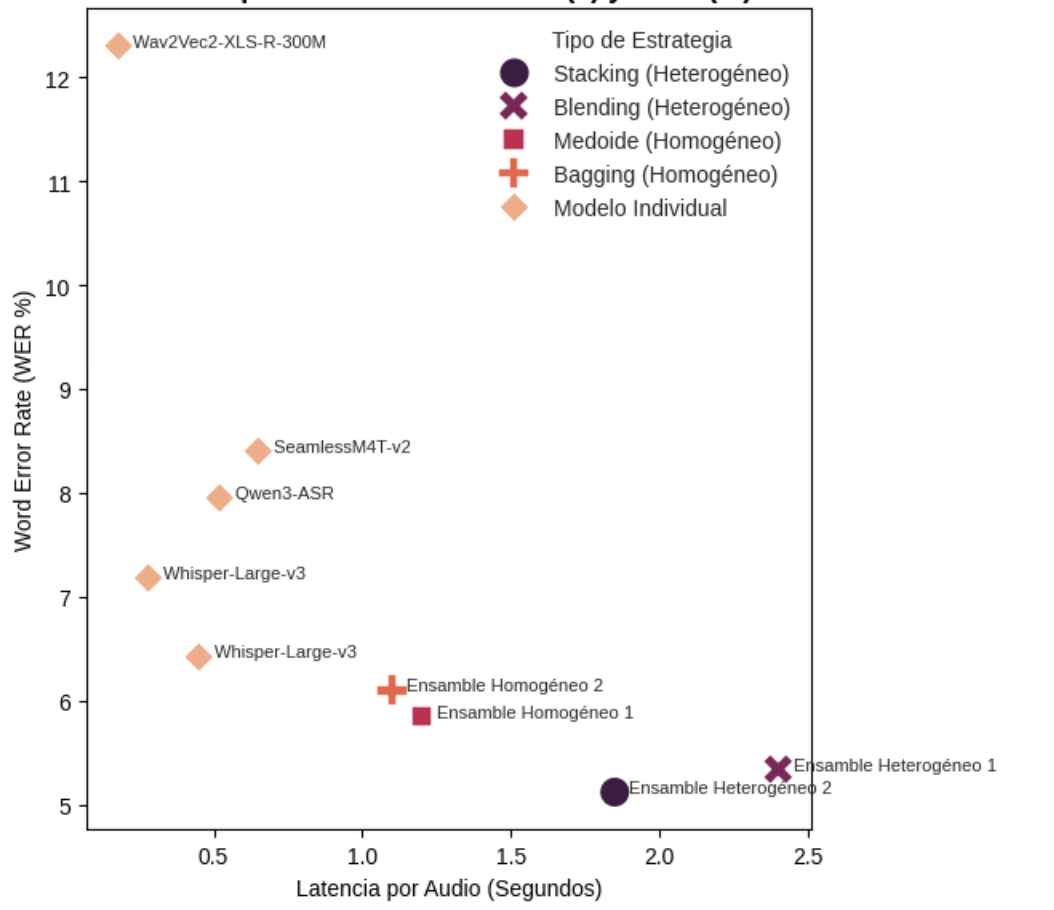
\includegraphics[width=0.85\textwidth]
    {latencia.png}
    \caption{Relación entre calidad y latencia para las configuraciones de decodificación comparadas.}
    \label{fig:latencia}
    \begin{minipage}{0.9\textwidth}
        \footnotesize
    \end{minipage}
\end{figure}

\subsection{Monitoreo y gobierno del modelo}
El monitoreo debe cubrir cuatro dimensiones:
\begin{enumerate}
\item \textbf{Operación:} disponibilidad, tasa de errores, latencia p50/p95/p99, profundidad de cola, throughput, GPU y VRAM.
\item \textbf{Calidad:} CER y WER en muestras etiquetadas, tasa de transcripciones vacías, longitud anómala, idioma detectado y tasa de revisión humana.
\item \textbf{Equidad:} métricas por idioma, familia de escritura, dialecto y otros metadatos disponibles; diferencias entre grupos.
\item \textbf{Datos:} cambios en duración, ruido, frecuencia de muestreo y distribución de idiomas respecto del conjunto de referencia.
\end{enumerate}

Como no existen transcripciones de referencia para cada solicitud en producción, la calidad real no siempre puede calcularse en línea. Se propone evaluación diferida sobre muestras consentidas y etiquetadas, además de auditorías periódicas con hablantes competentes. Las métricas automáticas de confianza deben validarse antes de usarse para decisiones.

\begin{table}[H]\centering
\caption{Indicadores operativos que deben registrarse.}
\begin{tabularx}{\textwidth}{lX}\toprule\textbf{Indicador} & \textbf{Uso}\\\midrule
Latencia p50, p95 y p99 & Verificar experiencia de usuario y cumplimiento de SLA.\\
CER/WER por idioma & Detectar degradación de calidad cuando existan referencias.\\
Tasa de error y reintentos & Identificar inestabilidad o fallas de integración.\\
GPU/VRAM y throughput & Dimensionar recursos y ajustar concurrencia.\\
Distribución de idiomas y duración & Detectar cambios de tráfico y datos fuera de distribución.\\
Brecha entre grupos & Evitar que una mejora global oculte deterioro en un idioma.\\
Tasa de derivación humana & Medir incertidumbre operacional y carga de supervisión.\\\bottomrule\end{tabularx}\end{table}

\section{Conclusiones}
El estudio permitió desarrollar un flujo de procesamiento reproducible de evaluación ASR y demostrar que la definición de métricas es parte central de la equidad lingüística. El hallazgo metodológico principal fue que WER no debe aplicarse uniformemente a idiomas sin segmentación por espacios. CER ofrece una comparación más adecuada a nivel de carácter, siempre que la normalización preserve particularidades ortográficas.

En la evaluación comparativa, Whisper-Large-v3 presentó el menor WER promedio reportado (4.39\%) entre los modelos individuales evaluados. La etapa de optimización y selección seleccionó la configuración greedy como referencia operativa y reportó 4.91\% CER, 8.03\% WER en idiomas con espacios y 1.491 segundos por audio. Estos resultados apoyan un piloto controlado, pero no justifican un despliegue universal ni autónomo. La evaluación de ocho idiomas y 80 muestras de prueba no cubre la variabilidad de acentos, dialectos, ruido y habla espontánea real.

La decisión de implementación es condicional: se recomienda proceder con un piloto supervisado y posponer el despliegue general en producción. Antes de liberar el servicio se deben corregir las excepciones de audios largos, repetir métricas desde un entorno controlado, ampliar la validación, definir umbrales por caso de uso, ejecutar pruebas de carga y establecer monitoreo de calidad y equidad. Si las brechas por idioma persisten, el proceso debe regresar a preparación de datos o modelación, en lugar de ocultar fallas mediante un promedio global.

Como líneas de investigación futura se proponen ampliar el benchmark a idiomas y dialectos prioritarios de CLEAR, incorporar audio espontáneo y condiciones acústicas reales, realizar comparaciones pareadas de modelos con el mismo protocolo, estudiar la relación entre disponibilidad de recursos lingüísticos, fertilidad de tokenización y errores, y evaluar adaptación o fine-tuning cuando exista un corpus representativo y autorizado. También se requiere documentar costos por minuto, capacidad concurrente y políticas de revisión humana. La contribución del estudio no consiste en declarar un modelo universalmente superior, sino establecer un proceso de evaluación transparente, reproducible y sensible a la diversidad lingüística.

\section*{Declaración de uso de herramientas de inteligencia artificial}
Durante el desarrollo de las etapas del estudio se documentó el uso de herramientas de IA para apoyar la estructuración de cuadernos computacionales, depuración de código y formulación de métricas y visualizaciones, y redacción técnica. En la etapa comparativa se documentó el uso de Claude y Gemini; en la etapa de optimización y selección se documentó el uso de ChatGPT. Para la elaboración y organización del presente manuscrito también se utilizó OpenAI ChatGPT, modelo GPT-6, como apoyo para integrar los documentos proporcionados, estructurar el texto y generar el código \LaTeX. Los autores deberán revisar, corregir y validar cada cifra, interpretación, referencia y decisión antes de entregar; la responsabilidad académica y aprobación corresponden a sus integrantes. La declaración deberá ajustarse para reflejar con precisión las herramientas y actividades efectivamente utilizadas por el equipo.

\begin{thebibliography}{99}
\bibitem{conneau2023} Conneau, A., Baevski, A., Richaud, A., et al. (2023). FLEURS: Few-shot learning evaluation of universal representations of speech. \textit{IEEE Open Journal of Signal Processing, 4}, 297--305. https://doi.org/10.1109/OJSP.2023.3263882
\bibitem{gebru2021} Gebru, T., Morgenstern, J., Vecchione, B., Vaughan, J. W., Wallach, H., Daumé III, H., \& Crawford, K. (2021). Datasheets for datasets. \textit{Communications of the ACM, 64}(12), 86--92. https://doi.org/10.1145/3458723
\bibitem{graham2024} Graham, C., \& Roll, N. (2024). Evaluating OpenAI's Whisper ASR: Performance analysis across diverse accents and speaker traits. \textit{JASA Express Letters, 4}(2), 025206. https://doi.org/10.1121/10.0024876
\bibitem{mitchell2019} Mitchell, M., Wu, S., Zaldivar, A., Barnes, P., Vasserman, L., Hutchinson, B., Spitzer, E., Raji, I. D., \& Gebru, T. (2019). Model cards for model reporting. In \textit{Proceedings of the Conference on Fairness, Accountability, and Transparency} (pp. 220--229). ACM. https://doi.org/10.1145/3287560.3287596
\bibitem{omnilingual2025} Omnilingual ASR Team, Keren, G., Kozhevnikov, A., et al. (2025). Omnilingual ASR: Open-source multilingual speech recognition for 1600+ languages. \textit{arXiv preprint arXiv:2511.09690}. https://arxiv.org/abs/2511.09690
\bibitem{radford2023} Radford, A., Kim, J. W., Xu, T., et al. (2023). Robust speech recognition via large-scale weak supervision. In \textit{Proceedings of the 40th International Conference on Machine Learning} (Vol. 202, pp. 28492--28518). PMLR. https://proceedings.mlr.press/v202/radford23a.html
\bibitem{shi2026} Shi, X., Wang, X., Guo, Z., Wang, Y., Zhang, P., et al. (2026). Qwen3-ASR technical report. \textit{arXiv preprint arXiv:2601.21337}. https://arxiv.org/abs/2601.21337
\bibitem{seamless2023} Seamless Communication, Barrault, L., Chung, Y.-A., et al. (2023). SeamlessM4T: Massively multilingual \& multimodal machine translation. \textit{arXiv preprint arXiv:2308.11596}. https://arxiv.org/abs/2308.11596
\bibitem{studer2021} Studer, S., Bui, T. B., Drescher, C., Hanuschkin, A., Winkler, L., Peters, S., \& Müller, K.-R. (2021). Towards CRISP-ML(Q): A machine learning process model with quality assurance methodology. \textit{Machine Learning and Knowledge Extraction, 3}(2), 392--413. https://doi.org/10.3390/make3020020
\bibitem{swain2024} Swain, M., van Zee, A. K., \& Søgaard, A. (2024). On mitigating performance disparities in multilingual speech recognition. In \textit{Proceedings of the 2024 Conference on Empirical Methods in Natural Language Processing}. Association for Computational Linguistics. https://aclanthology.org/2024.emnlp-main.323/
\bibitem{tabassi2023} Tabassi, E. (2023). \textit{Artificial intelligence risk management framework (AI RMF 1.0)} (NIST AI 100-1). National Institute of Standards and Technology. https://doi.org/10.6028/NIST.AI.100-1
\bibitem{thennal2025} Thennal, D. K., James, J., Gopinath, D. P., \& Ashraf, M. K. (2025). Advocating character error rate for multilingual ASR evaluation. In \textit{Findings of the Association for Computational Linguistics: NAACL 2025}. Association for Computational Linguistics. https://aclanthology.org/2025.findings-naacl.277/
\bibitem{vanzee2024} van Zee, A. K., van Zee, M., \& Søgaard, A. (2024). Group fairness in multilingual speech recognition models. In \textit{Findings of the Association for Computational Linguistics: NAACL 2024} (pp. 2213--2226). Association for Computational Linguistics. https://doi.org/10.18653/v1/2024.findings-naacl.143
\end{thebibliography}

\appendix
\small
\setstretch{1.0}
\renewcommand{\arraystretch}{1.0}


\section{Tablas de resultados desagregados por idioma}
La tabla siguiente deberá completarse con resultados extraídos del CSV definitivo del experimento. Se mantiene sin completar deliberadamente para evitar inferir métricas que no aparecen consolidadas en los entregables. Añadir una fila por idioma y especificar el tamaño de muestra.
\begin{longtable}{p{0.20\textwidth}r r r r}
\caption{Plantilla para resultados finales desagregados por idioma.}\\
\toprule Idioma / código & $n$ & CER (\%) & WER (\%)$^*$ & Latencia (s)\\\midrule
\endfirsthead
\toprule Idioma / código & $n$ & CER (\%) & WER (\%)$^*$ & Latencia (s)\\\midrule
\endhead
Idioma 1 (por completar) & & & & \\
Idioma 2 (por completar) & & & & \\
Idioma 3 (por completar) & & & & \\
Añadir una fila por cada idioma evaluado & & & & \\
\bottomrule
\end{longtable}
\small $^*$Reportar WER solo cuando la segmentación por espacios sea lingüísticamente válida; en caso contrario indicar N/A y explicar la métrica alternativa.

\begin{figure}[H]
    \centering
    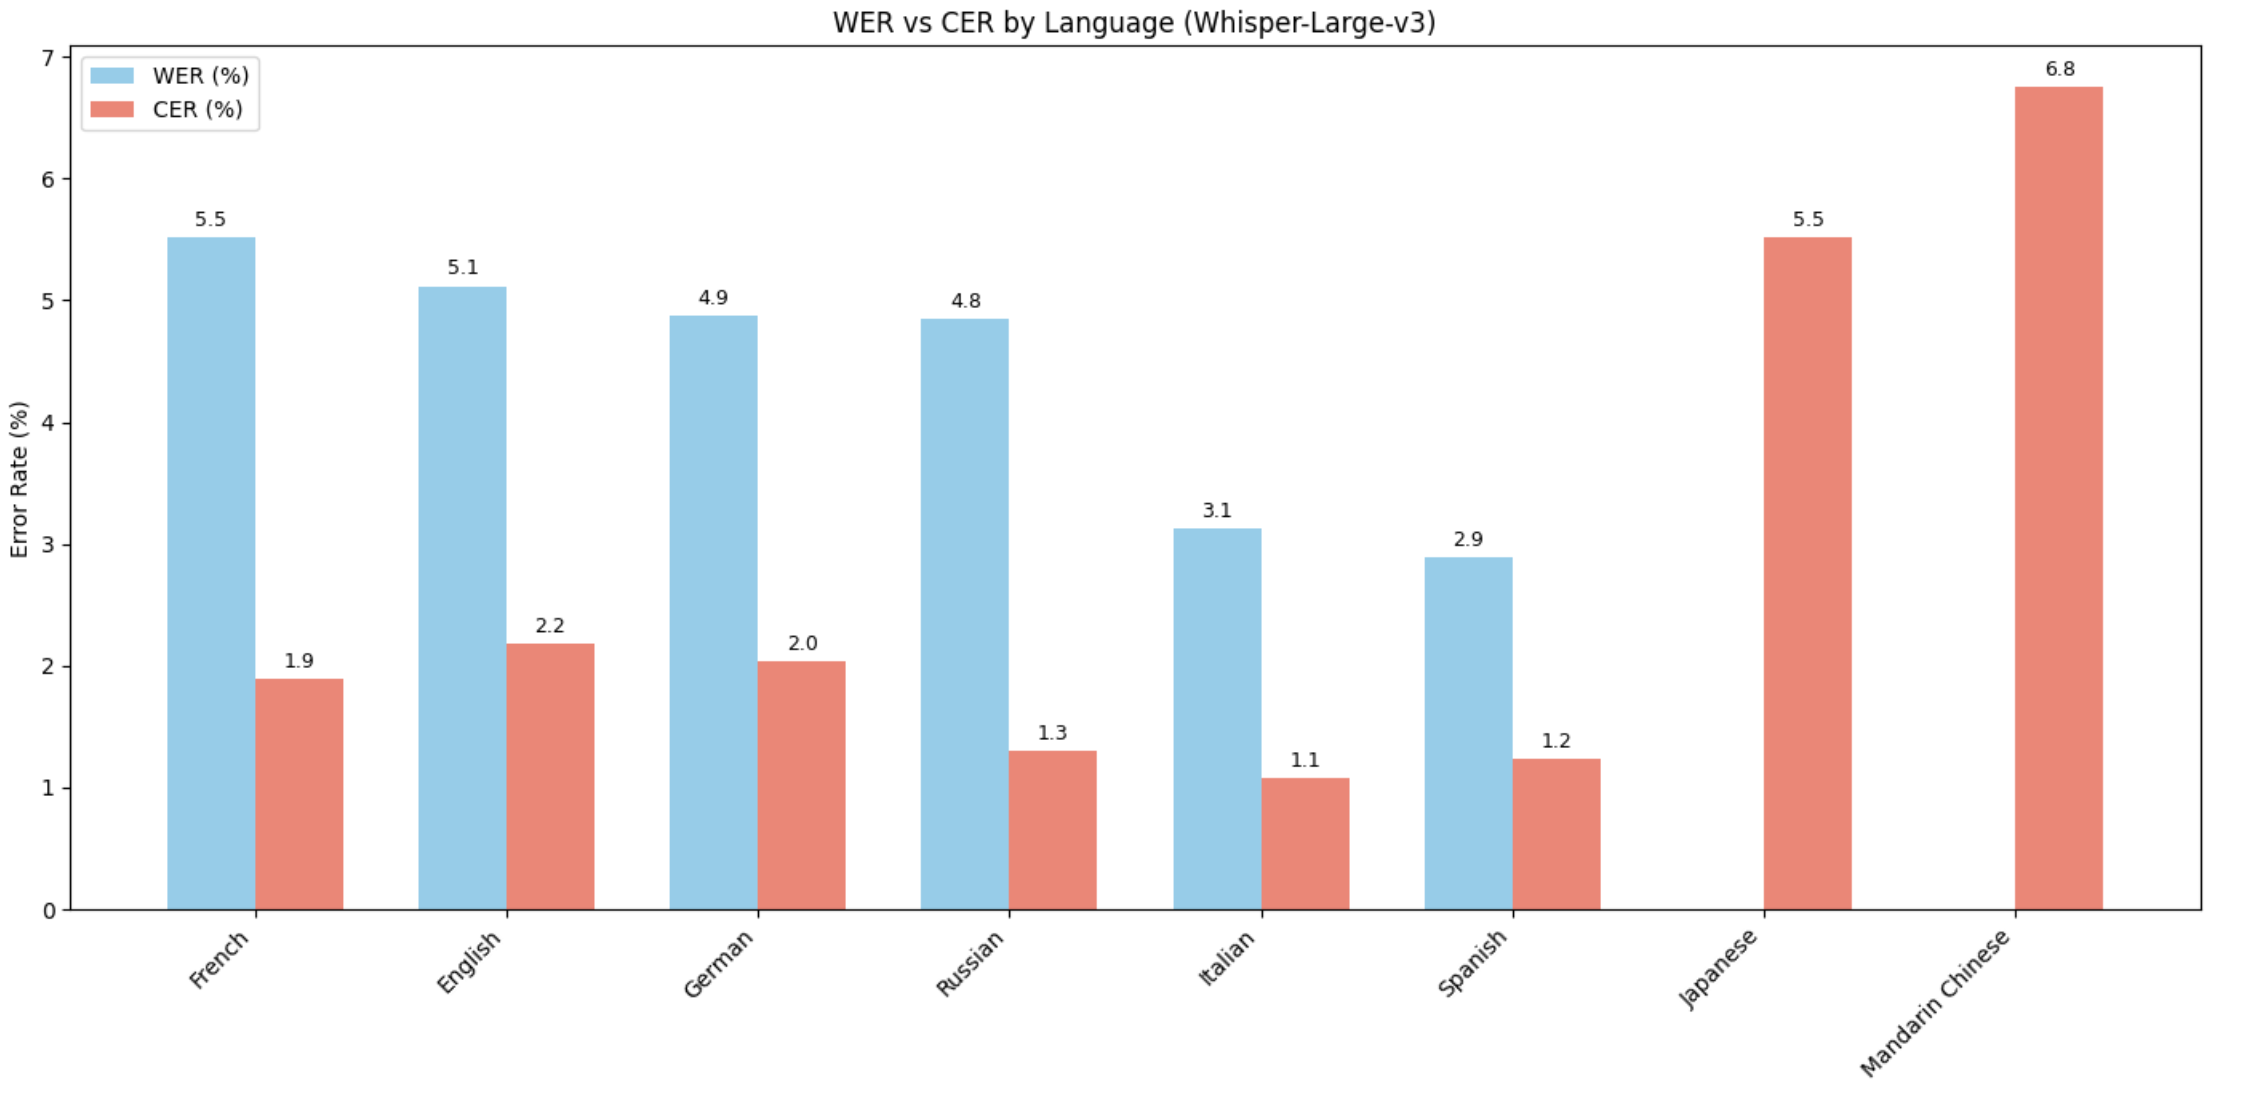
\includegraphics[width=0.85\textwidth]
    {whisper_metricas.png}
    \caption{Resultados desagregados de CER y WER por idioma para el modelo final.}
    \label{fig:latencia}
    \begin{minipage}{0.9\textwidth}
        \footnotesize
    \end{minipage}
\end{figure}


\section{Arquitectura de referencia y controles de operación}
La figura de arquitectura presentada en el cuerpo del artículo sintetiza el flujo lógico propuesto. Para el diseño de implementación, completar además los siguientes controles:
\begin{itemize}
\item \textbf{Entrada:} autenticación, autorización, límites de tamaño/duración, validación de MIME y protección contra archivos malformados.
\item \textbf{Procesamiento:} cola con límite de concurrencia, almacenamiento temporal cifrado, borrado según política y trazabilidad de transformaciones.
\item \textbf{Inferencia:} imagen de contenedor inmutable, pesos identificados por hash, GPU dimensionada con pruebas de carga y estrategia de fallback.
\item \textbf{Salida:} transcripción, idioma, versión del modelo, estado de procesamiento y advertencia cuando el idioma o la calidad estén fuera del alcance validado.
\item \textbf{Observabilidad:} métricas de servicio p50/p95/p99, throughput, errores, cola, VRAM y calidad diferida por idioma cuando existan referencias.
\item \textbf{Gobierno:} responsable del modelo, calendario de auditoría, proceso de incidentes, rollback y revisión de cambios de datos/modelo.
\end{itemize}

\section{Ficha resumida del modelo y límites de uso}
El modelo evaluado en la etapa de optimización y selección es exclusivamente \texttt{openai/whisper-large-v3}; las configuraciones greedy, Beam Search y medoide son estrategias de inferencia sobre esa misma arquitectura, no modelos base diferentes.
{\scriptsize
\setlength{\tabcolsep}{3pt}
\renewcommand{\arraystretch}{0.88}
\begin{longtable}{p{0.27\textwidth}p{0.63\textwidth}}
\textbf{Elemento} & \textbf{Contenido por completar / declarar}\\\hline
Nombre y versión & Whisper-Large-v3; registrar checkpoint y hash.\\
Uso previsto & Transcripción asistida en idiomas y escenarios aprobados para el piloto.\\
Usos no autorizados & Alto impacto sin revisión humana; idiomas no evaluados; usos fuera de dominio.\\
Datos de evaluación & FLEURS y muestra de la etapa de optimización y selección; documentar particiones, licencias y representatividad.\\
Desempeño & Métricas macro, micro y por idioma; intervalos de confianza cuando sea posible.\\
Sesgos y limitaciones & Variación por idioma, escritura, acento, dialecto, canal y tipo de habla.\\
Supervisión & Revisión humana, corrección y abstención/fallback.\\
Mantenimiento & Versionado, monitoreo, regresión y revisión periódica.\\
\end{longtable}
}

\section{Artefactos, gráficas y reproducibilidad}
Repositorio: \url{https://github.com/Luz026/VoiceBenchmark}. Para reproducir el estudio, conservar commit, hashes de datos, configuración, dependencias, hardware, particiones y CSV. Insertar las gráficas PNG en \texttt{figuras/}, junto al archivo \texttt{.tex}, usando los nombres indicados en los recuadros; regenerar las cifras antes de la entrega final.
\end{document}
